% vim: tw=80 cc=81 spelllang=cs spell

% XXX: Remove 'draft' in final version
% XXX: Remove 'oneside' and 'openany' for printed version
\documentclass[11pt, a4paper, oneside, openany, draft]{book}

% Input and output encoding
\usepackage[utf8]{inputenc}
\usepackage[T1]{fontenc}

% XXX: Guess what to change if you intend to write in English
\usepackage[english]{babel}

\usepackage[usenames,dvipsnames]{xcolor}
\usepackage{lmodern}
\usepackage{enumitem}
\usepackage{todonotes}
\usepackage{setspace}
\usepackage{graphicx}
\usepackage{amssymb,amsmath}
\usepackage{mathtools}
\usepackage{float}
\usepackage[pass]{geometry}
\usepackage{ifdraft}

% Theorems – add your own environments, should you need them.
\usepackage{amsthm}
\newtheorem{theorem}{Věta}

% Source code listings
\usepackage[draft=false]{minted}
\usemintedstyle{friendly}
\newminted{hs}{autogobble,linenos}

% Algorithms
\usepackage[Algoritmus]{algorithm}

\usepackage[ unicode=true,
             plainpages=false,
             pdfpagelabels,
             draft=false,
             hyperfootnotes=false,
             colorlinks=true,   % XXX: for PDF
             %colorlinks=false, % XXX: for print
             %hidelinks,        % XXX: for print
             linkcolor={Sepia},
             citecolor={PineGreen},
             urlcolor={MidnightBlue},
           ]{hyperref}

% XXX
\hypersetup{
    pdfauthor={Samuel Malec},
    pdftitle={Side effect analysis},
    pdfsubject={Master thesis}
}

\usepackage[backend=bibtex8,
            sortlocale=cs_CZ, % XXX
            bibencoding=UTF8
            maxnames=100
           ]{biblatex}
% XXX: Add your bibliography to bibliography.bib
\addbibresource{bibliography.bib}

\setlength{\tabcolsep}{6pt}

% Macros for linking sections suitable for use in Czech text.
% e.g., v \myref{somelabel}{sekci} → v sekci 5.2
%       v \ymref{somelabel}{kapitole} → v 5. kapitole
\newcommand{\myref}[2]{\hyperref[#2]{#1~\ref*{#2}}}
\newcommand{\ymref}[2]{\hyperref[#1]{\ref*{#1}.~#2}}

% % % % % % % % % % % % % % % % % % % % % % % % % % % % % % % % % % % % % % % % 

\begin{document}
\frontmatter
% XXX: Go edit titlepage.tex
\newgeometry{margin=3cm,top=7cm}
\pagestyle{empty}

\begin{center}
    {\Large \textsc{Masaryk university}}

    {\large \textsc{faculty of informatics}}
    \vskip4em
    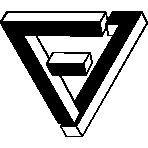
\includegraphics[width=4cm, height=4cm, draft=false] {logo_fi.pdf}
    \vskip4em
    {\begin{spacing}{1}
        \Huge \textbf{Side effect\\analysis} % XXX: Title
    \end{spacing}}
    \vskip2em
    {\Large \textsc{master thesis}} % XXX: Type
    \vskip2em
    {\LARGE \textbf{Samuel Malec}} % XXX: Author
    \vfill
    {\hfill\large Brno, 2026} % XXX: Year
\end{center}

\cleardoublepage
\restoregeometry

% XXX: Go edit frontmatter.tex
\frontmatter
\pagestyle{empty}

\vspace*{4em}

\begin{center}
    {\Large \textsc{Masaryk University}}

    {\large \textsc{Faculty of Informatics}}
    \vskip4em
    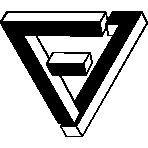
\includegraphics[width=4cm, height=4cm]{logo_fi.pdf}
    \vskip4em
    {\begin{spacing}{1}
        \Huge \textbf{Side-Effect Analysis Using a Static Single Use Program Representation}
    \end{spacing}}
    \vskip2em
    {\Large \textsc{Master's Thesis}}
    \vskip2em
    {\LARGE \textbf{Samuel Malec}}
    \vfill
    {\hfill\large Brno, 2026}
\end{center}

\cleardoublepage
\strut
\cleardoublepage

\section*{Declaration}
I hereby declare that this thesis is my original work and that I developed it
independently. I have properly cited all sources and literature used in this
thesis and provided complete references to them.

\vfill
\textbf{Supervisor:} TBD 

\cleardoublepage

\section*{Acknowledgements}
Write your acknowledgements here.

\cleardoublepage

\section*{Abstract}
Write your abstract here.

\bigskip
\subsection*{Keywords}
keyword, keyword

\cleardoublepage

\pagestyle{plain}
\setcounter{tocdepth}{1}
\tableofcontents

\mainmatter
\pagestyle{scrheadings}


\setcounter{tocdepth}{2}
\tableofcontents
\pagestyle{plain}

\mainmatter
% XXX: Organise your chapters however the fuck you like
% vim: spell spelllang=cs
\chapter{Úvod}

Protože trend rozežraných webových stránek už svoji lehce vulgární odpověď
má~\cite{web:mf}, rozhodl jsem se v~podobném duchu ukázat, že \LaTeX ová kostra
závěrečné práce může existovat v~analogicky jednoduché podobě.

,,Fakulta``\footnote{orgán, který neexistuje (až by si
v~něm člověk objednal nápoj (za osm korun))} od pradávna
shilluje svým studentům šablonu \texttt{fithesis}, která sice už podle názvu
zní, že je \emph{the perfect fit for the job} a~slibuje, že všechny náležitosti
bakalářky a~diplomky vyřeší za vás, ale je neestetická, nevzhledná, hnusná;
škaredá i~šeredná; ohyzdná, ohavná, odporná i~otřesná a~nádavkem ještě k~zblití.

Prozradím vám teď tajemství: na sazbu své sračky, za niž chcete dostat titul,
nepotřebujete žádnou zázračnou externí šablonu; všechno co potřebujete, jste si
nainstalovali se základním \LaTeX ovým balíkem. (Pomiňme teď Overleaf; jestli
nutně potřebujete cpát každé usrání do obláčku, určitě to někdo časem překlopí
i~tam.)

Možná jste nabyli dojmu, že ten fithesistní nevkus vás aspoň zbaví některých
starostí s~\TeX em, a~že je to tedy skvělá volba, pokud jste studovali nějaký
odpadní obor, během něhož jste na tento osmdesátkový klenot nemuseli sahat.
Špatně! Je to úplně stejný krám jako zbytek \LaTeX ového světa, akorát se k~němu
ještě trochu hůř kachní\footnote{basic bitches si můžou doplnit ,,googlí``}
rovnáky na ohýbáky, protože nevíte, které narovnání nedopatřením ohnete uvnitř
šablony, o~níž zbytek světa jaktěživ neslyšel (šťastné to lidstvo).

Zahoďte tedy obavy, vy\TeX at bakalářku zvládli větší lempli než vy a~příkazy na
formátování obsahu jsou úplně stejné pro fithesi jako tady, v~relativně čistém
\LaTeX ovém \texttt{book}. Na ten zbytek máte tuhle kostru, která ale nic
divnějšího nepoužívá a~hlavně vám všechno odhaluje a~umožňuje změnit přímo, bez
nějakých pomocných maker nebo sahání kdoví kam.

Nechci tu tvrdit, že \texttt{book} je kdovíjaký typografický skvost, na druhou
stranu na předčení úrovně fithese stačí žalostně málo. Jestli vám na
estetičnosti sazby fakt záleží (což v~době elektronicky odevzdávaných prací
popravdě ztrácí na významu) a~z~\LaTeX u strach nemáte, \emph{prosím}, všemi
deseti sáhněte po něčem hezčím (osobně mám rád šablonu
\texttt{mimosis}\footnote{\url{https://github.com/Pseudomanifold/latex-mimosis}}).
Tenhle počin je odpovědí na argument „já s~tím lateksem neumím a~ta fithesis už
má všechno nastavené, tak to bude nejlepší volba“. Není. Jestli máte celou
bakalářku tak na háku, že byste použili fithesi, použijte radši tohle -- bude to
mít úplně stejný „žádný velký sraní“ vajb, ale ve výsledku to bude  vypadat líp.

% vim: spell spelllang=cs
\chapter{Použití kostry}

Je to tak triviální, až se z~toho člověku obklopenému všemožnými bloated
nesmysly chce brečet.

\begin{enumerate}
    \item Stáhněte si kostru do adresáře na závěrečnou práci.
    \item Otevřete \texttt{thesis.tex} a~vyhledávejte text \texttt{XXX}, jímž
    jsou označeny části, které určitě budete chtít upravit.
    \begin{itemize}
        \item Surprise twist! Části \texttt{XXX} vás mohou poslat do jiných
        souborů, v~nichž se nachází jiné části \texttt{XXX}, které budete chtít
        upravit! Říká se tomu rekurse a~je to princip a~nástroj, bez jehož
        pochopení se do psaní své nezáživné práce možná radši ani nepouštějte.
        \item Chcete změnit něco, co nemá \texttt{XXX}? Nelíbí se vám můj výběr
        barev? Toužíte po jiných okrajích? No tak to změňte, ta kostra se z~toho
        (asi) neposere.\footnote{ono teda co v~\LaTeX u se sem tam „samo“ neposere}
    \end{itemize}
    \item Obsah si narvěte, kam chcete; já navrhuji podadresář
    \texttt{chapters}. Jistě pochopíte, kam ho v~hlavním souboru zařadit.
    Přiložený makefile s~tím trochu počítá, ale přiložený makefile není svatý
    a~upravit ho zvládnete i~se znalostmi z~PB152cv nebo kde se to teď učí.
    \begin{itemize}
        \item Při vkládání literatury chcete do \texttt{bibliography.bib}
        yoinknout to, co se se jmenuje \emph{záznam BibTeX} nebo nějak podobně.
    \end{itemize}
    \item Jestli máte \texttt{latexmk}, tak už stačí \texttt{make} nebo (pro
    živé přesazování) \texttt{make pvc}.
    \item Před odevzdáním povypínejte pracovní věci (hlavně režim
    \texttt{draft}).
\end{enumerate}

Odtud už to zvládnete sami, že?

\section{Příklady}

Jestli nezvládnete, tak přichází část s příklady použití, které zároveň slouží
jako ukázka pro to příkladové PDFko, na které se pravděpodobně zrovna díváte.
Nakonec, i já na něčem musím vyzkoušet, že věci nevypadají úplně hnusně.

Nicméně není to úvodem do \LaTeX u. Jestli sháníte něco takového, zkuste
Wikibooks~\cite{wb}.

\subsection{Seznamové struktury}

Použité příklady by možná chtěly nějaký delší text, ale číslovaný seznam
s odstavci máte o kousek výš a do odrážkového seznamu možná odstavce dávat
nechcete?

\begin{itemize}
    \item raz,
    \item dva,
    \item tři:
    \begin{itemize}
        \item ča,
        \item ča.
    \end{itemize}
\end{itemize}

Čísla se vrství do písmen, což jde nějak změnit a ta Wikikniha~\cite{wb} vám
snad i~řekne, jak.

\begin{enumerate}
    \item posbírat kalhotky
    \item ???
    \item \textsc{Získat}
    \begin{enumerate}
        \item povšimnout si existence kapitálek (angl.~\emph{small caps}),
        \item používat je, protože verzálky vprostřed textu jsou trochu fuj.
    \end{enumerate}
\end{enumerate}

Nevím, jestli jsem v životě viděl nějak rozumně použitý seznam definic, ale
budiž. Sám jsem ho použil akorát jako \texttt{\textbackslash paragraph}
s odsazením.

\begin{description}
    \item[tvaroh] vynikající mléčný výrobek
    \item[ráfek] část kola, na niž se navléká pneumatika
\end{description}

\subsubsection{Členění textu}

Sekce, podsekce a podpodsekce (což je tato) nejsou technicky seznamová
struktura, ale v obsahu tak v podstatě fungují. Ve výchozím nastavení se do
obsahu promítají nadpisy jen po úroveň podsekce, ale lze to změnit -- hledejte
\texttt{tocdepth} v hlavním souboru.

\paragraph{Odstavec}
Potřebujete-li oddělit ještě menší úsek textu, existují i „nadepsané“ odstavce
a dokonce pododstavce, což jsou technicky pořád odstavce, ale jejich nadpis se
snaží tvářit, že ještě pod něco patří. Nepovažuji to úplně za typografický
zázrak, ale třeba se to někam může hodit a nepůsobit moc škaredě.

\subparagraph{Pododstavec}
Toto je pododstavec. Podle mě je úplně hnusný a potřebujete-li nějaký použít,
myslím, že byste se měli vrátit o pár kroků výš a zkusit text rozčlenit jinak.
Ale tak co já vím, nesežral jsem moudrost světa.

\bigskip
Mimochodem, ten černý obdélník na kraji indikuje \emph{přetok} -- text, který se
nepodařilo rozumně zalomit. Řeší se přeformulováním věty (nebo i některé
předchozí), či v případě divných slov ručním na\-zna\-če\-ním slo\-vo\-děl\-by,
které by se mohl \TeX\ chytit.


\subsection{Figury}

Je to tak, pořád netuším, jak přeložit slovo ,,figure``, které zahrnuje obrázky,
tabulky i útržky zdrojového kódu sedící trochu mimo hlavní tok textu. Můžete je
zabalit do plovoucího prostředí, což znamená, že s ním \TeX\ může různě hýbat,
nebo je můžete nechat vykreslit přímo v místě definice.

Připravte se na to, že cokoli plovoucího může být boj a rozbíjet sazbu, kdežto
cokoli neplovoucího může být boj a rozbíjet sazbu. Ohledně nastavení plovoucího
prostředí se informujte třeba zase v té Wikiknížce~\cite{wb}, dá se tomu říkat,
jaké umístění to má preferovat a tak.

\subsubsection{Tabulky}

Tohle je velké a bolestivé téma, přikládám proto jen jednoduchou ukázku
(\myref{tabulka}{tab:example}) nějakých výsledků vycucaných z prstu. Miliardu
různých možností najdete ve~\cite{wb}.

\begin{table}
    \centering
    \begin{tabular}{l | r r r r | r}
        zařízení       &  firmware & loader & kernel & userspace & celkem \\\hline
        \texttt{nymfe} &     4,5~s &  2,5~s &  3,0~s &      10~s & 17,0~s \\
        \texttt{musa}  &     2,5~s &  1,5~s &  2,0~s &       8~s & 14,0~s
    \end{tabular}
    \caption{Rychlost startování fakultních počítačů}
    \label{tab:example}
\end{table}

\subsubsection{Zdrojáky}

Tohle nebude o moc menší boj. Můžete použít obstarožní \texttt{listings}, které
jsou trochu otravné na nastavení, ale na pár jednoduchých útržků kódu fungují
dostatečně. Popsáno je to nečekaně ve~\cite{wb} a ještě nečekaněji pak někde
v dokumentaci toho balíku.

Modernější, barevnější a na sazbu pomalejší varianta je \texttt{minted}, který
pro změnu potřebuje pythonový balíček \texttt{pygmentize} a povolit \TeX u
spouštět externí programy volbou \texttt{-shell-escape}, ale výsledek je pak
podle mě hezčí a snáze se přidávají kódy ve více programovacích jazycích. Ten
používám v~této kostře.

\begin{minted}{latex}
% Je možné automaticky zavést prostředí s přednastavením
\newminted{hs}{autogobble,linenos}
\begin{hscode}
    main :: IO ()
    main = readLine >>= putStrLn
\end{hscode}
\end{minted}

Dává:

\begin{hscode}
main :: IO ()
main = readLine >>= putStrLn
\end{hscode}

\subsubsection{Obrázky}

Co by to bylo za takypráci bez komixů z Visual Paradigm a screenshotu webového
prohlížeče! Protože se mi nechtělo přikládat zbytečné obrázky jen pro účely
příkladu, najdete na \myref{obrázku}{fig:example} jen to, co už jste viděli na
titulní straně. Tedy, v režimu \texttt{draft} spíš nenajdete.

\begin{figure}[H]
    \centering
    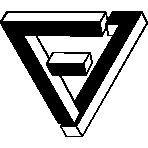
\includegraphics[height=4cm]{logo_fi.pdf}
    \caption{Adamatova představa o logu fakulty. Toto není v žádném případě
    oficiální logo, ale protože to staré ustrnulo v roce 99 a to nové je
    najbrtshit, bylo opět nutno přistoupit k věci proaktivně a ohnout si realitu
    podle vlastní vůle.}
    \label{fig:example}
\end{figure}

Lze si povšimnout, že na rozdíl od tabulky jsem požádal o umístění obrázku
mezi odstavci, což má jisté estetické problémy a neměl jsem to dělat. Také je
možné si povšimnout, že tabulky a obrázky se číslují zvlášť.

\subsubsection{Algoritmy}

Pokud nechcete vkládat přímo zdroják, ale strukturovaný popis algoritmu
v~pseudokódu, má na to \LaTeX samozřejmě taky nějaké balíčky.
\myref{Algoritmus}{alg:example} je vysázen pomocí ???\todo{Najít dobré
algoritmítko}.

\begin{algorithm}[H]
TODO
\caption{Řazení sléváním}
\label{alg:example}
\end{algorithm}

\subsection{Matematika}

Dokonce i na \textsc{fi mu} se občas v závěrečných pracích vyskytne potřeba
sázet výrazy, rovnice nebo jinou matiku. K tomu bych přišoupnul ještě prostředí
na lemmátka, věty a důkazy. Opět se běžte podívat na tu Wikiknihu~\cite{wb}.

\begin{theorem}
    Algoritmus \ref{alg:example} běží v $\mathcal{O}\left(\sqrt{n^2}\cdot\log n\right)$.
\end{theorem}
\begin{proof}
    No jen se na něj podívejte!
\end{proof}

No a pak se samozřejmě hodí sazba zarovnaných rovnic. A~jestli pak
chcete na některé z rovnic odkazovat v textu, fakt si otevřete~\cite{wb}.

\begin{align*}
D &= b^2 - 4\cdot a \cdot c\\
x_{1,2} &= \frac{-b\pm\sqrt{D}}{2}
\end{align*}

Hledáte-li makro pro sazbu konkrétního symbolu, zkuste použít
Detexify\footnote{\url{https://detexify.kirelabs.org/classify.html}}.

\appendix
\chapter{Archív s implementací}

Něco něco elektronická verze práce\footnotemark\todo{Doplnit isové id práce}
něco něco archiv s implementací. Něco něco soubory:

\begin{itemize}
    \item \texttt{src/} se samotným zdrojovým kódem,
    \item \texttt{doc/} s uživatelskou dokumentací a
    \item \texttt{README} obsahující další pokyny.
\end{itemize}

\footnotetext{Dostupná na adrese \url{https://is.muni.cz/th/XXXXX}}


\backmatter
\chapter{Literatura}
\begingroup
\raggedright
\printbibliography[heading=none]
\endgroup

\ifoptiondraft{\listoftodos}

\end{document}
